\documentclass[conference]{IEEEtran}
\usepackage{amsmath,amssymb,amsfonts}
\usepackage[usenames,dvipsnames]{xcolor}
\usepackage{tikz, pgfplots, pgfplotstable}
\usepgfplotslibrary{units}
\usetikzlibrary{patterns}
\usetikzlibrary{tikzmark}
\usetikzlibrary{graphs}
\usepgfplotslibrary{colorbrewer}
\pgfplotsset{%
  compat = newest,%
  table/search path = {data},%
  % Common bargraph style
  my bargraph colors/.style = {%
    colormap/Paired,%
    cycle list = {%
      {index of colormap={0}, fill=., draw=.},%
      {index of colormap={1}, fill=., draw=.},%
      {index of colormap={2}, fill=., draw=.},%
      {index of colormap={3}, fill=., draw=.},%
      {index of colormap={4}, fill=., draw=.},%
      {index of colormap={5}, fill=., draw=.},%
      {index of colormap={6}, fill=., draw=.},%
      {index of colormap={7}, fill=., draw=.},%
      {index of colormap={8}, fill=., draw=.},%
    },%
  },%
  my bargraph style/.style = {%
    axis on top,%
    axis lines* = left,%
    major grid style = {%
      draw = white,%
    },%
    my bargraph colors,%
    area legend,%
    reverse legend,%
    legend style = {%
      draw=none,%
    },%
  },%
  % xbar specific
  my xbar style/.style = {%
    xbar = 0pt,%
    bar width = 6pt,%
    xmajorgrids,%
    xtick distance = 1,%
    major x tick style = { draw=none, },%
    major x grid style = { white, },%
    my bargraph style,%
    tickwidth = 0pt,%
    x axis line style = {%
      opacity = 0,%
    },%
    xticklabels = {\empty},%
    y axis line style = {%
      draw = black,%
    },%
    To change tick font sizes:
    every tick label/.append style = {%
      font=\footnotesize{},%
    },%
    ytick = data,%
    %  Text entries:
    y dir = reverse,%
    visualization depends on=rawx\as\rawx,%
    nodes near coords = {%
      \footnotesize{}\pgfmathprintnumber{\rawx}%
    },%
  },%
  polybench speedup style/.style = {%
    width=1.0\textwidth,%
    height=4cm,
    enlarge x limits = { abs = 1em, },%
    y axis line style = {%
      opacity = 5,%
    },%
    %enlargelimits=0.02,%
    % bar settings
    bar width=5pt,%
    % Y axis settings
    ybar=0.5pt,%
    ymajorgrids,
    ytick distance = 50,%
    ymajorticks=true,%
    % X axis settings
    xtick pos=bottom,%
    % xtick=data,%
    % legend settings
    legend pos=north east,%
    %legend columns=-1,%
    legend cell align={left},%
    legend style={font=\small},%
    every axis plot/.append style={fill},%
    cycle list/Accent,% color setting look for colorbrewer
  },%
  customOp speedup style/.style = {%
    height=7cm,
    enlarge x limits = { abs = 1em, },%
    y axis line style = {%
      opacity = 0,%
    },%
    %enlargelimits=0.02,%
    % bar settings
    bar width=8pt,%
    % Y axis settings
    ytick pos=left,%
    ybar=0pt,%
    ymajorgrids,
    ytick distance = 1,%
    ymajorticks=true,%
    % X axis settings
    xtick pos=bottom,%
    xtick=data,%
    xticklabel style = { rotate = 60, anchor = east, font=\small },%
    x label style={at={(axis description cs:0.5,-0.28)},anchor=north},%
    % legend settings
    legend pos=north west,%
    %legend columns=-1,%
    legend cell align={left},%
    legend style={font=\small},%
    every axis plot/.append style={fill},%
    cycle list/Accent,% color setting look for colorbrewer
  },%
}
\pgfplotstableset{%
  col sep=comma,%
}
\pgfplotsset{compat=1.11,
    /pgfplots/ybar legend/.style={
    /pgfplots/legend image code/.code={%
       \draw[##1,/tikz/.cd,yshift=-0.25em]
        (0cm,0cm) rectangle (3pt,0.8em);},
   },
}

\begin{document}

    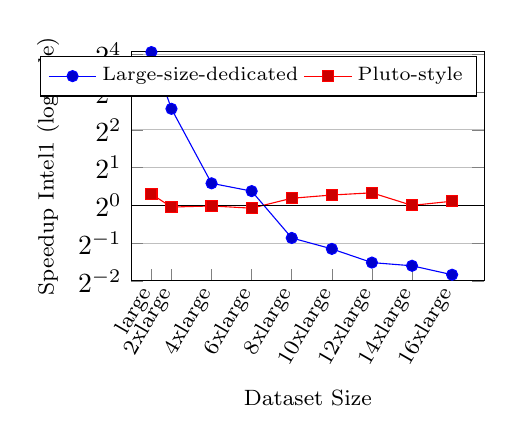
\begin{tikzpicture}%
      \begin{axis}[%
        %Sizes
        width=0.5\textwidth,%
        height=4.5cm,
        %Y axis settings
        ymin = 0.25,%
        ymax = 17,%
        ylabel=Speedup Intel1 (logscale),%
        ylabel style = { font=\footnotesize },
        xlabel style = { font=\footnotesize },
        %Ticks settings
        ytick distance = 2,%
        xtick=data,%
        xtick pos=bottom,%
        xticklabel style = { rotate = 60, anchor = east, font=\footnotesize },%
        xticklabels = {large, 2xlarge, 4xlarge, 6xlarge, 8xlarge, 10xlarge, 12xlarge, 14xlarge,         16xlarge},%
        xmin=0,%
        %Legend Settings
        legend cell align={left},%
        legend style={font=\scriptsize},%
        legend columns=-1,
        %General Settings
        xlabel=Dataset Size,%
        ymode=log,%
        log basis y={2},%
        ymajorgrids,%
      ]%

        \addplot 
	      coordinates {(1,16.69) (2,5.89) (4,1.50) (6, 1.30) (8,0.55) (10, 0.45) (12, 0.35) (14, 0.33) (16,0.28)};

        \addplot 
	      coordinates {(1,1.23) (2,0.97) (4,0.99) (6, 0.95) (8,1.14) (10, 1.21) (12, 1.26) (14, 1.00 ) (16,1.08)};

        \draw [black] (axis cs:-1,1) -- (axis cs:20,1);%

        \addlegendentry{Large-size-dedicated};%
        \addlegendentry{Pluto-style};%
      \end{axis}%
    \end{tikzpicture}

\end{document}